\subsection{Proposed solution}

With the aim of providing a way for researchers to focus on the development of
their solution, rather than the collection of a dataset, and to produce a
theoretically infinite amount of possible circuit configurations, a
semi-synthetic dataset generation is proposed, and further put to the test.

Semi-synthetic images of mixed reality have been used in the past, as mentioned
previously with the work of Cheung \etal~\cite{CheungWBM17}, but required a
complex pipeline of algorithms to produce a visually coherent image. The
disposition of a motion capture system at Aarhus Deep Tech, capable of
providing millimeter precision with its twelve cameras, makes it very easy to
recreate a virtual camera in the exact same configuration as the one capturing
the background images.

This valuable asset, added to the limited time available to develop the
solution, motivates the choice of using annotated base images, despite their
limitations.\\

The idea proposed for the aforementioned solution is to generate a virtual
scene representing randomly positioned virtual gates that a drone would
potentially have to fly through in the real world. A rendered image of the said
scene is then overlaid onto a real image, taken from the drone's camera, as to
represent a random portion of a racing circuit, as seen from the drone's field
of view. 

\begin{figure}[h]
	\center
	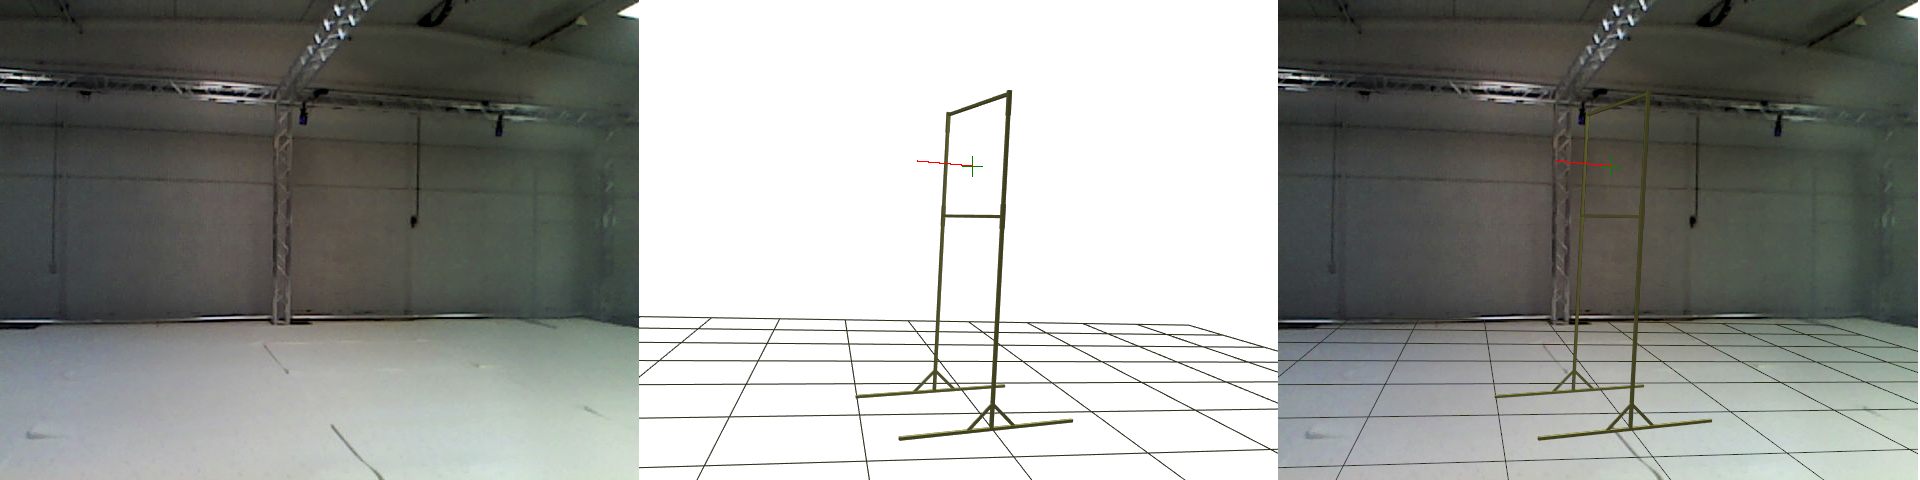
\includegraphics[width=\textwidth]{figure/dataset_solution.png}
	\caption[The steps of a semi-synthetic image generation.]{A decomposition
	of the making of a semi-synthetic image, representing randomly positioned
	3D models of randomly selected gates overlaid on top of a randomly selected
	real-world background image. The virtual scene's camera is positioned and
	oriented using the exact configuration of the background image, so that
	both perspectives match. The perspective grid is kept for visualization
	purposes.}
\end{figure}

In order to do so, several requirements have to be met.\\

Firstly, a motion capture system, such as the ones used in the movie production
industry, is used to record the position and orientation of the drone in 3D
space, also known as the extrinsic parameters of the camera. This is crucial
for the generation of a virtual scene whose perspective matches to the
perfection the perspective of the drone, so that the generated scene can later
be overlaid onto the real scene.

Secondly, the virtual camera must be a perfect model of the actual camera used
to capture the background images, since the perspective calculation is derived
from its intrinsic parameters. Therefore, the drone camera needs to be
calibrated in order to estimate its parameters, before being able to apply
them to the virtual camera.

Finally, the dimensions of the virtual scene must be in accordance with the
actual dimensions of the physical space where the dataset of background images
was recorded, otherwise unwanted artifacts such as gates being visible outside
the confinement of the real scene could be produced. The same reasoning can be
applied to the 3D models of gates or obstacles, since their scale most likely
matters for the usage of the generated images.\\

	\subsubsection{Advantages}

As previously stated, the main advantage of being able to generate a dataset of
semi-synthetic images lies in the freedom of choice for the 3D models to be
rendered, and in the annotations that can be generated along with them.

Furthermore, because each scene is generated by projecting a random selection
of available meshes, along with a random choice of texture (consider a color),
in a random configuration, the hypothesis is that each new image represents a
unique case which a drone could potentially face in the real world.

Another non-negligible  advantage is the possibility to artificially set the
brightness and contrast of the resulting image, thus offering even more
adaptation potential to the CNN.\\

%Based on those facts, 

	\subsubsection{Limitations}

In spite of the numerous assets this solution has, it poses limitations,
notably in regard to data augmentation and choice of environment.

Indeed, since a motion capture system is needed to record the pose of the
drone, it is not possible to record a background dataset in any external
environment.

Moreover, because the ground truth labels depend on the position of the nearest
gate in the image, it heavily dampers the possible image augmentation
techniques. The latter is often used in the case of limited data samples for
the training phase, which is not the case here since an infinite amount of
images can be generated, in theory.

It would still be possible to apply image transformations such as image shift,
vertical or horizontal flip, shearing and other augmentations, but the ground
truth would have to be recomputed with respect to the transformation, which can
be difficult to do.
